\chapter{The LHCb experiment}
\label{ref:detector}

The LHCb experiment is one of the four large experiments (CMS, ATLAS, ALICE,
LHCb) at the Large Hadron Collider (LHC),
a superconducting circular proton-proton collider (mostly\footnote{
    Heavy ions are also collided at the LHC,
    but are not relevant for this analysis.
}), built and managed by
the European Organization for Nuclear Research (CERN),
with a center of mass energy
$\sqrt{s} = 13$~TeV during its run 2 (2016--2018) operation period.

Located 100 meters underground at Franco-Swiss border,
the LHCb detector,
shown in \cref{fig:lhcb-detector},
is a forward only spectrometer covering the pseudorapidity\footnote{
    Defined as the following:
    $\eta \equiv -\ln\left[\tan\left(\frac{\theta}{2}\right)\right]$,
    with $\theta$ the angle between the 3-momentum of a particle
    and the positive direction of the beam axis.
}
range $1.9 < \eta < 4.9$,
with a focus on the $b$- and $c$-physics precision measurements.
% coverage of bbbar
The unusual geometry of the LHCb detector
(as opposed to $4\pi$ detectors with full solid angle coverage,
for example the other three large experiments at the LHC)
is largely driven by the \bbbar production mechanism at the LHC:
the dominant production mode is gluon fusion in which case the momenta of the
incoming partons are highly asymmetric in the laboratory frame.
As a result, the \bbbar center of mass is boosted either forward or backward
in the beam direction \cite{Altarelli_2008},
as confirmed by simulation of \bbbar production angular distribution,
shown in \cref{fig:bbbar-prod-angular}.
With just about 4\% solid angle coverage,
the LHCb detector efficiently and economically reconstructs about 20\%
of all produced \bbbar pairs \cite{Belyaev_2021}.

\begin{figure}[!htb]
    \centering
    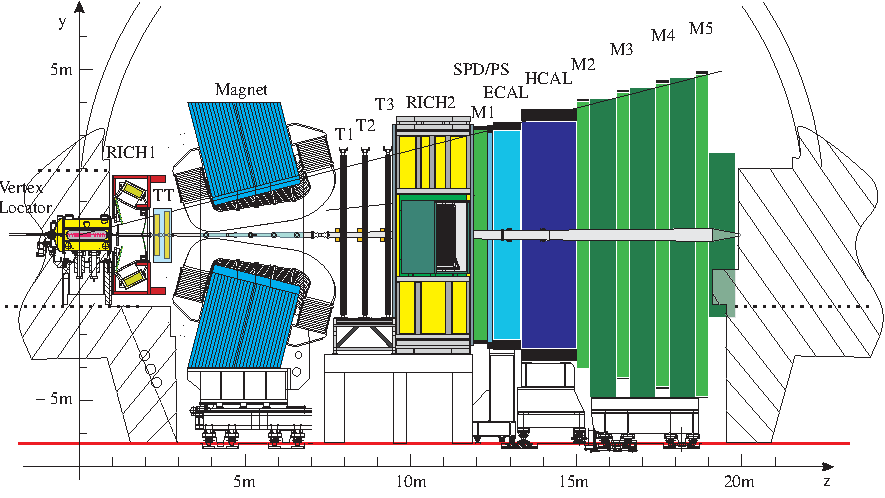
\includegraphics[width=0.95\textwidth]{./figs-detector/lhcb_detector_view.pdf}
    \caption{
        The LHCb detector.
        $z$ axis indicates \bbbar travelling direction.
        The impact point is at $z = 0$.
    }
    \label{fig:lhcb-detector}
\end{figure}

\begin{figure}[!htb]
    \centering
    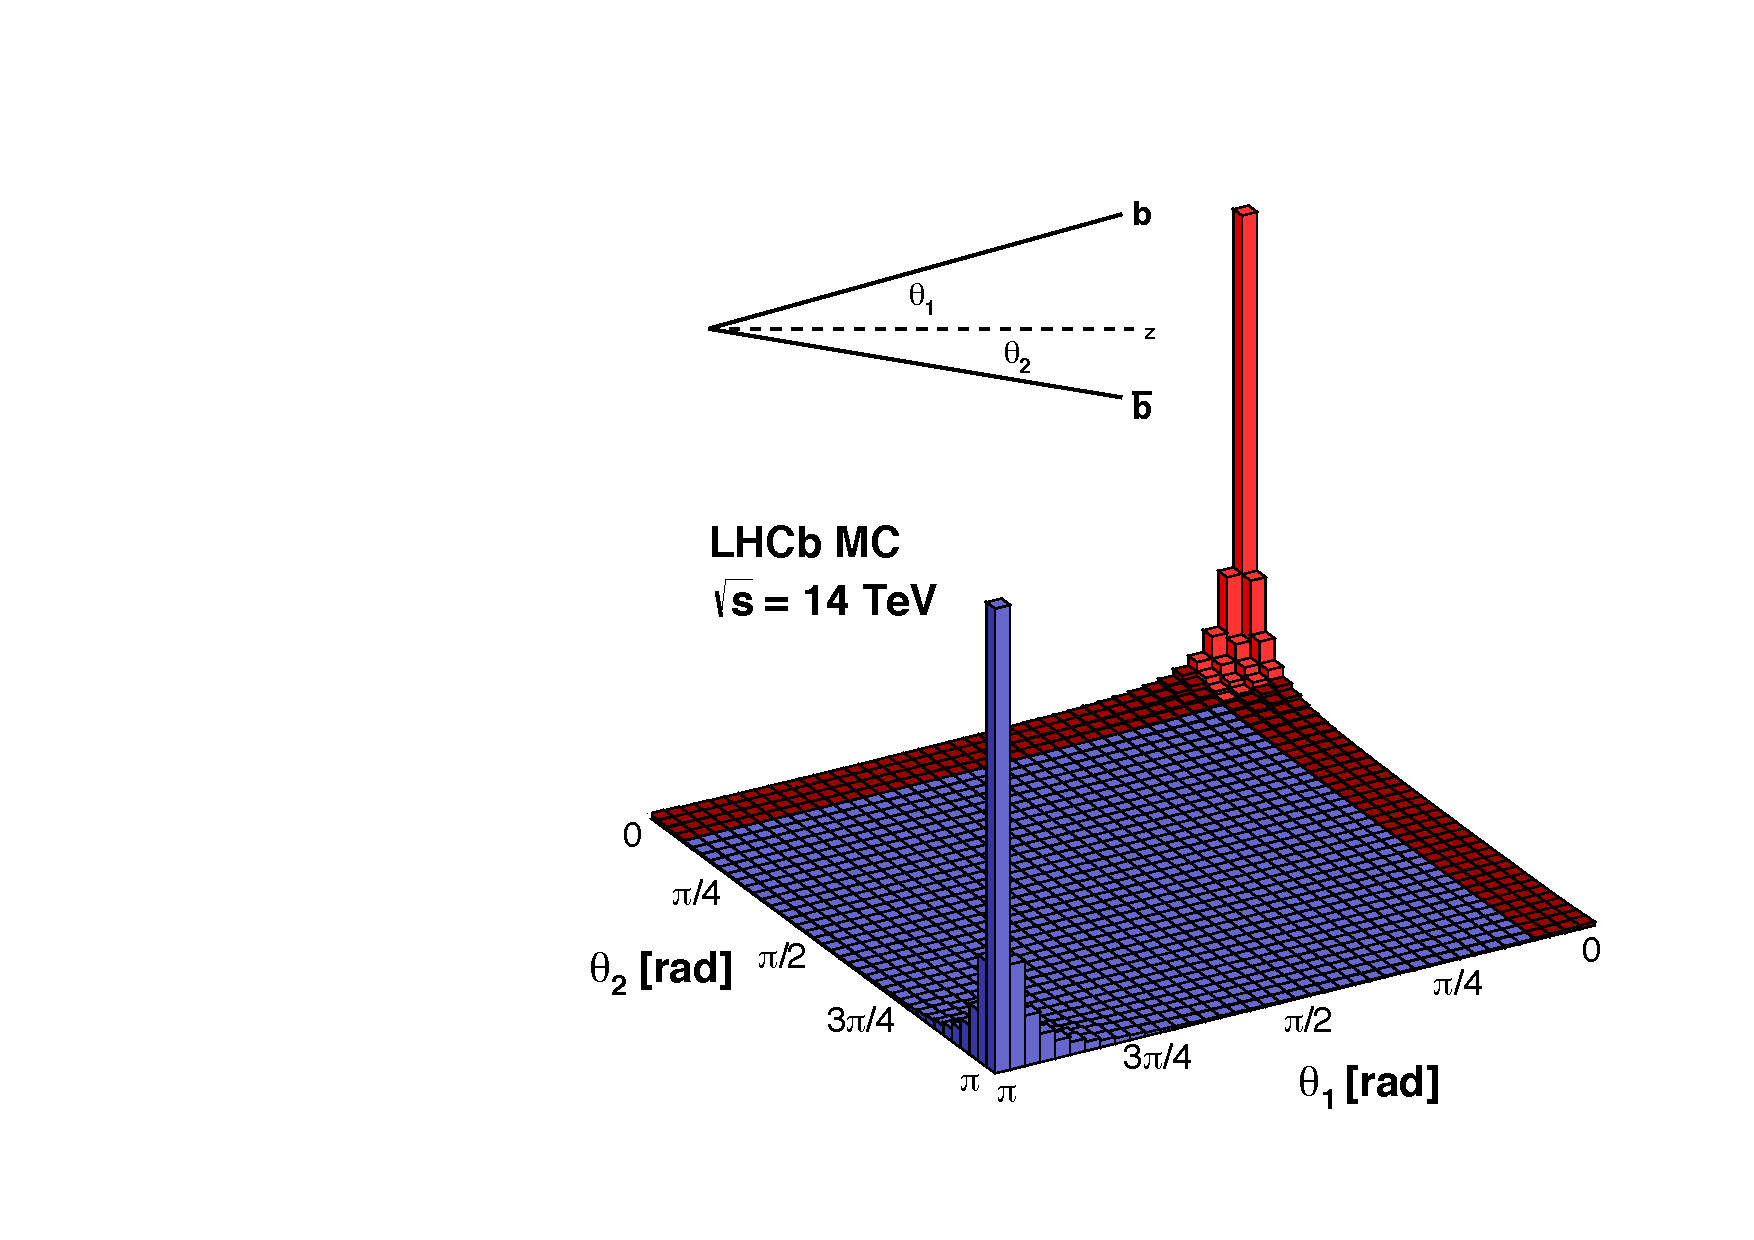
\includegraphics[width=0.6\textwidth]{./figs-detector/14_rad_acc_scheme_right.pdf}
    \caption{
        Simulated \bbbar production angular distribution at $\sqrt{s} = 14$ GeV.
        Taken from \cite{LHCb_bb_prod_angle}.
    }
    \label{fig:bbbar-prod-angular}
\end{figure}

% luminosity run 1+2
At the designed LHC luminosity, multiple $pp$ collisions happen within the
same bunch crossing (an effect called ``pile up'')
which greatly complicates \bbbar production and event reconstruction because
the event\footnote{
    An event is defined as \emph{everything} produced in a single bunch
    crossing.
} is significantly more \emph{busy}
(compared to events with single $pp$ collision)
\cite{Altarelli_2008}.
To maintain the luminosity at optimal values for LHCb,
a technique termed \emph{luminosity levelling} is implemented to dynamically
\emph{defocus} beams by offsetting them in the transverse direction based
on reported LHC instantaneous luminosity
\cite{https://doi.org/10.5170/cern-2014-004.183}.
%%%%
Over the course of run 1 and 2 operation periods, LHCb recorded a total
integrated luminosity of $\sim 8.7$~fb$^{-1}$
\cite{LHCb_lumi},
corresponding to over 300 billion $B$ mesons and several billions of other
$b$ hadrons,
an unprecedented number for $b$-physics.
% NOTE: The lumi is not unprecedented as BaBar achieved 411 ifb.

In general, the LHCb detector has the following features,
all of which required by $b$-physics measurements:
a precise tracking system providing excellent track and vertex resolution;
a good particle identification performance separating \pion, \kaon, $e$, \muon,
and $p$ (proton);
a versatile trigger scheme efficient for both hadron and lepton
with lower \pt thresholds\footnote{
    Compared to CMS and ATLAS, but the lepton trigger \pt threshold is still too
    high for this analysis.
}.
The rest of chapter provides a brief introduction for the subdetectors of the
LHCb detector relevant for this analysis, grouped by the features listed above.
An overview of reconstruction of charged particles is provided in
\cref{ref:detector:tracking};
particle identification is described in \cref{ref:detector:pid};
the basics of trigger implementation is explained in
\cref{ref:detector:trigger}.


\section{Reconstruction of charged particles}
\label{ref:detector:tracking}

Charged particle reconstruction relies on the tracking system,
which consists of the following components
(sorted based on the proximity from the $pp$ interaction point):

\begin{itemize}
    \item VErtex LOcator (VELO):
        it is a compact 21-layer silicon-strip detector placed immediately
        around the $pp$ interaction point\footnote{
            The first few layers (stations) are located upstream the interaction
            point (backward direction),
            whereas the last layers are downstream (forward direction).
        }
        \cite{The_LHCb_Collaboration_2008}
        that detects particles with a pseudorapidity ranging from
        $1.6 < \eta < 4.9$.
        Each layer of VELO,
        made of two retractable\footnote{
            This is required because the VELO sensors are placed 8~mm from the
            LHC beam.
            The gap is smaller than the aperture required by the beam during
            injection,
            so the semi-disks are retracted in such cases.
        } silicon half disks with a pitch\footnote{
            ``Pitch'' refers to the size of a single silicon strip, akin to a
            ``pixel'' in the LCD screen.
            A smaller pitch generally implies a better resolution.
        } ranging from 37 to 98~$\upmu$m (increasing with radius),
        provides radial and azimuthal angular position measurements of a track.
        Combining positional information from all layers (with a fit),
        a tracking resolution of about 4~$\upmu$m at best is achieved
        \cite{Aaij_2014}.
        The primary vertex (PV) resolution depends on number of tracks (nTracks)
        used in vertex reconstruction,
        ranging from 35--10~$\upmu$m in the transverse plane
        (low nTracks to high),
        and 260--60~$\mu$m in the beam axis.

    \item Tracker Turicensis (TT):
        located downstream of VELO and immediately before the Magnet,
        the TT consists of 4 planes of silicon-strip sensors,
        each of a size 150~cm $\times$ 130~cm,
        with a strip pitch of 183~$\upmu$m arranged in a straight/stereo
        configuration\footnote{
            This will be explained in \cref{ref:ut:overview}.
        }.
        It covers the full acceptance of the LHCb experiment, and has a spatial
        resolution of about 50~$\upmu$m
        \cite{The_LHCb_Collaboration_2008}.

    \item T-stations:
        they are located immediately downstream of the Magnet.
        There are a total of 3 T-stations with a common design.
        Each of them is made up of two subdetectors: The Inner Tracker (IT),
        covering a cross-shaped region around the beam pipe,
        and the Outer Tracker (OT),
        covering the rest of the LHCb acceptance.
        The IT is made of silicon strips (same technology as in TT) whereas the
        OT uses gas-tight straw-tubes.
        The IT has a spatial resolution identical to that of TT,
        namely 50~$\upmu$m.
        For the OT, its resolution is about 205~$\upmu$m
        \cite{OT_2014}.
\end{itemize}

Due to the design of the LHCb detector, tracks are approximately straight lines
separately in the upstream and downstream (in terms of the Magnet) segments
because of a lack of magnet field.
The downstream and upstream segments,
labelled as VELO tracks and T-tracks,
are first reconstructed separately before attempting to match them to form long
tracks.
If compatible hits are found in the TT during the matching,
they are added to the track to further improve the momentum resolution and
reduce the amount of fake tracks (ghosts).
Different track types are shown in \cref{fig:track-types}.
In most analyses, this one included, only long tracks are used because they
provide the best momentum resolution
\cite{LHCb-DP-2013-002}.

\begin{figure}[!htb]
    \centering
    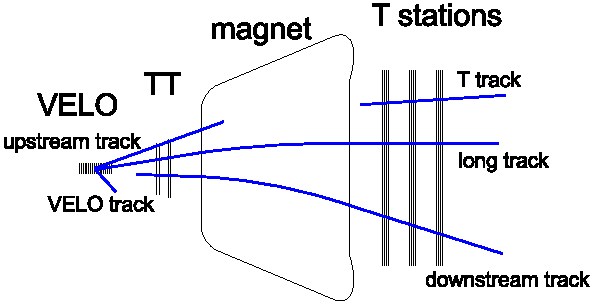
\includegraphics[width=0.75\textwidth]{./figs-detector/tracking/track_type.pdf}
    \caption{
        Reconstructed track types at LHCb.
    }
    \label{fig:track-types}
\end{figure}


\section{Particle identification}
\label{ref:detector:pid}

The particle identification (PID) system consists of three subsystems:

\begin{itemize}
    \item Two Ring Imaging CHerenkov (RICH) detectors:
        RICH1 and RICH2.
        The former is situated between the VELO and the TT,
        the latter after the T-stations.
        The RICH detectors provide identification for charged hadrons,
        with limited discrimination power for $e$ and \muon.
        These two detectors measure the Cherenkov angle of emitted photons from
        charged particles traversing through the medium,
        which depends on its refractive index $n$,
        the momentum $p$ of the particle, and the mass $m$ of the particle:

        \begin{equation}
            \theta_c = \frac{\sqrt{1 + (m/p)^2}}{n}
        \end{equation}

        Particles with different masses result in different Cherenkov angles.
        At sufficiently large momentum,
        Cherenkov angles saturate and can no longer tell different particles
        apart.
        To ensure good PID performance across a wider range of momentum,
        materials with different refractive indices are used in RICH1 and RICH2.

        RICH1 uses a gas layer of $\text{C}_4 \text{F}_{10}$ with $n = 1.0014$.
        This material provides hadron identification from about 1 to 60~GeV,
        and covers the full LHCb acceptance.
        RICH2 has a smaller angular acceptance corresponding to a region enriched
        of high-momentum particles.
        It uses a $\text{C}\text{F}_{10}$ gas radiator with $n = 1.00046$,
        providing PID up to 150~GeV
        \cite{Belyaev_2021}.
        In \cref{fig:rich-plots}, Cherenkov angles of different particles are
        shown; it also displays a real measurement of Cherenkov angles from
        RICH1.

    \item A calorimeter system:
        composed of 4 subdetectors:
        the Scintillator Pad Detector (SPD), the Preshower Detector (PS),
        the Electromagnetic CALorimeter (ECAL),
        and the Hadron CALorimeter (HCAL).
        Located downstream of the T-stations, the calorimeter system measures
        energy deposit from all particles.
        Combining information from the tracking system,
        it can determine the presence of $e, \gamma$ and neutral
        hadrons:
        $e$ leaves a trajectory in the tracking system, while depositing most
        of its energy in ECAL;
        $\gamma$ is invisible to tracking but deposits most energy in ECAL;
        while also invisible to the tracking system,
        neutral hadrons deposit energy in both ECAL and HCAL
        \cite{Belyaev_2021}.
        Note that PID in calorimeters is a destructive measurement:
        All particles except muons and neutrinos deposit all their energy
        in the calorimeters by producing electromagnetic or hadronic showers
        \cite{Lippmann_2012}.

        All calorimeters are made of segments of scintillators with different
        granularity,
        with ECAL and HCAL having multiple layers of alternating scintillators
        and absorbers.
        The calorimeters detects light from scintillators,
        emitted by particles travelling through,
        using photomultipliers as a way to measure energy deposit.

        The SPD and PS are two layers of scintillators separated by a 12~mm
        thick lead sheet.
        They are designed to indicate the presence of charged particles to the
        L0 calorimeter trigger.

        The ECAL employs the \emph{Shashlik} technology\footnote{
            The name comes from the fact that detectors constructed this way
            have similar appearances to a shashlik.
        } with 66 layers of
        independent modules constructed from 2~mm of lead plates followed by
        4~mm of scintillating material with Wave-Length
        Shifting (WLS) optical fibers piercing through the layers and guiding
        scintillating light to photomultipliers.
        The energy resolution for the ECAL is:

        \begin{equation}
            \frac{\sigma(E)}{E} = \frac{10\%}{\sqrt{E}} \oplus 1\%
        \end{equation}
        where $E$ is the electron energy in GeV.

        The HCAL consists of layers of iron absorber with scintillating tiles as
        the active material.
        Compared to ECAL, HCAL has a coarser granularity with a reduced
        energy resolution:

        \begin{equation}
            \frac{\sigma(E)}{E} = \frac{(69 \pm 5)\%}{\sqrt{E}} \oplus
            (9 \pm 2)\%
        \end{equation}
        where $E$ is the hadron energy in GeV.

    \item Five muon stations:
        Labelled as M1--M5, M1 is located in front of the calorimeter system
        whereas M2--M5 come after.
        Each muon station is of rectangular shape and made up by 1368
        multi-wire proportional chambers supplemented by 12 triple GEM chambers
        in the inner region of the first station \cite{Belyaev_2021}.
        The muon stations have an acceptance in the bending plane from
        20~mrad to 306~mrad and from 16~mrad to 258~mrad in the non-bending
        plane, resulting in a total acceptance of about 20\% for muons from
        semileptonic inclusive $b$ decays.

        The muon stations provide space point measurements
        as well as timing measurements of the remaining tracks,
        the vast majority of them being muons as most other particles,
        charged or uncharged,
        are absorbed by the detector before reaching the stations.
        By requiring muon-like particles to produce hits in certain muon
        stations in a momentum-dependent way\footnote{
            The actual requirement can be looked up from Table 1 of
            \cite{LHCB-DP-2013-001}.
        },
        a binary muon PID decision, \isMuon, is produced.
\end{itemize}

\begin{figure}[!htb]
    \centering
    \begin{subfigure}[t]{0.45\textwidth}
        \centering
        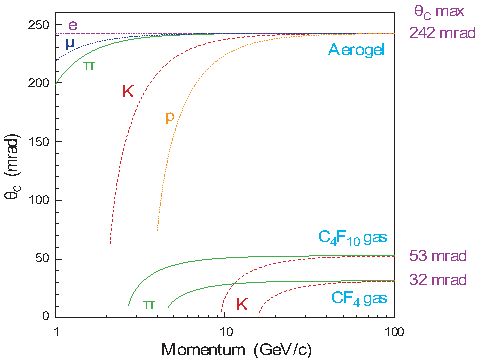
\includegraphics[width=\textwidth]{./figs-detector/pid/cherenkov_angle_media.pdf}
        \caption{
            Cherenkov angles for different particles traversing different media.
            ``Aerogel'' is irrelevant for run 2.
        }
    \end{subfigure}
    \hspace{12pt}
    %%%%
    \begin{subfigure}[t]{0.45\textwidth}
        \centering
        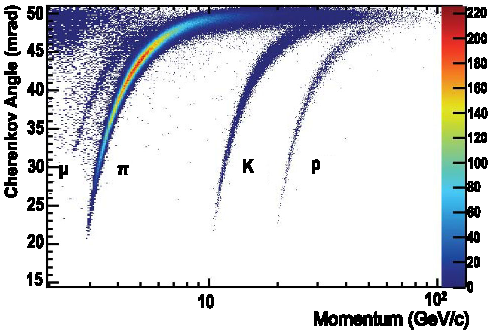
\includegraphics[width=\textwidth]{./figs-detector/pid/rich1_measurement.pdf}
        \caption{Cherenkov angles measured by RICH1.}
    \end{subfigure}

    \caption{
        PID in RICH detectors.
    }
    \label{fig:rich-plots}
\end{figure}

As a summary, the PID system exploits the fact that different types of
particles leave different signatures in the detectors,
schematically shown in \cref{fig:pid-signature},
to identify charged hadrons and leptons, as well as neutral hadrons.
Overall, the LHCb experiment provides two types of PID variables
\cite{Seuthe:2021fcn}:

\begin{itemize}
    \item DLL$_X$:
        These variables are the log likelihood difference between $X$ and \pion,
        with the log likelihoods combined from all three PID subsystems
        (RICH, calorimeters, muon stations):
        $\mathcal{L} = \mathcal{L}_\text{RICH} \cdot \mathcal{L}_\text{Calo}
        \cdot \mathcal{L}_\text{Muon}$.

    \item ProbNN$_X$:
        These variables are outputs from neural networks (NN) trained to
        identify $X$.
        The training inputs are from both the PID and the tracking system,
        with data-driven corrections from calibration samples.
\end{itemize}

\begin{figure}[!htb]
    \centering
    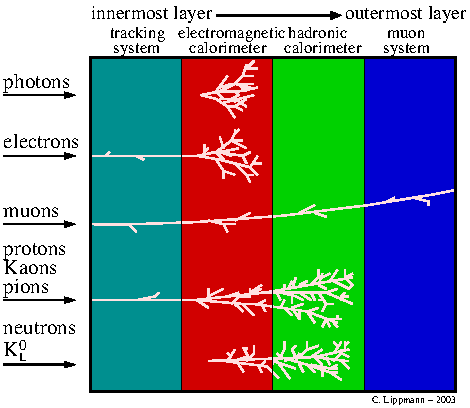
\includegraphics[width=0.5\textwidth]{./figs-detector/pid/pid_signatures.pdf}
    \caption{
        Signatures of different particles in a typical configuration
        of a modern detector.
        Taken from \cite{Lippmann_2012}.
    }
    \label{fig:pid-signature}
\end{figure}


\section{Trigger}
\label{ref:detector:trigger}

Despite the fact that the LHCb experiment operates at reduced luminosity,
it is still impractical to record the total output of all events due to readout
rate and storage limitations.
%%%%
The readout rate is first reduced from 40~MHz,
the LHC bunch crossing frequency,
to 1~MHz by hardware triggers,
referred to as Level-0 (L0) triggers.
The L0 triggers reconstruct transverse energy $E_T$ and momentum $p_T$ in real
time and select events with large $E_T$ or $p_T$,
a signature of $B$ meson decays due to their large masses.
In addition,
the number of $pp$ interactions in the event and the number of tracks are
estimated and events with large pile-up or multiplicity are rejected.
The reconstruction of these high-multiplicity events would require a
disproportionally large fraction of readout bandwidth and typically results in
poorer tracking quality.
%%%%
The selected events are further reconstructed by software high-level
triggers (HLT1 and HLT2) and only events with high-\pt tracks and/or large
impact parameters are further filtered with pre-defined cuts before being
retained on disk for offline analysis.
The HLT triggers reduce the output rate to about 12.5~kHz
\cite{Dordei:2017rtt}.

One of the main objective of the ongoing detector upgrade is to increase the
bandwidth of the detector readout thus removing the need of hardware triggers,
and all the limitations that come with them.
This section is dedicated to discussion of the hardware triggers (L0) which,
while no longer are a part of the LHCb run 3 program,
are of crucial importance to this analysis.
The high-level triggers will be discussed and compared between run 2 and run 3
with more details in \cref{ref:lhcb-upgrade-overview:trigger}.

The L0 trigger is divided into three components, with each connected to a
detector and its information collected by the Level-0 Decision Unit to evaluate
a final trigger decision, as shown in \cref{fig:l0-schematic}:

\begin{itemize}
    \item Pile-up system:
        located upstream of VELO, the pile-up system consists of two sets
        silicon disks of the same type used in VELO.
        It is the only detector that can estimate the track multiplicity
        in the backward direction.
        The intended use of the system was to veto events with multiple $pp$
        interactions but is unused because efficient high level triggers
        made pile-up less harmful \cite{Oggero:1635658}.
        As a reference, for run 1, the average pile-up is about 1.7;
        for run 2, it is about 1.1
        \cite{d_Argent_2017}.

    \item Calorimeter trigger system:
        it identifies the cluster
        ($2 \times 2$ cells of scintillators) with the largest
        $E_T$ and provides a PID decision (hadron, electron, or photon) of the
        cluster based on the calorimeter system only.
        The required $E_T / p_T$ threshold is set differently
        for each particle type.
        This analysis uses L0 hadron trigger which has a $E_T$ threshold
        of 3.7~GeV for year 2016 \cite{LHCb-DP-2019-001}.

        In addition, the total number of SPD cells with a hit is counted to
        estimated number of tracks (charged particles) in the event.
        Typically events are required to have fewer than 450 SPD hits.

    \item Muon trigger system:
        The muon stations can provide an independent measurement of the track
        \pt with a resolution of about 25\% on average
        \cite{LHCb-DP-2019-001}.
        The L0 muon triggers require that either the largest muon \pt exceeds
        1.8~GeV or the product of the two largest muon \pt exceeds 2.25~GeV$^2$
        (both are 2016 thresholds).

        As we will discuss in \cref{ref:sel:data:rs},
        this analysis \emph{relies} on uniform muon selection efficiency across
        \pt spectrum
        as low-\pt muons are a signature of the signal decays,
        whereas high-\pt muons typically come from normalization decays.
        Hence, the muon trigger cannot be used because it not only actively
        rejects signal, but also makes the selection efficiencies between signal
        and normalization different,
        which void the premise that measuring \RDX is preferred because
        experimental efficiencies are partially cancelled in the ratios.
\end{itemize}

\begin{figure}[!htb]
    \centering
    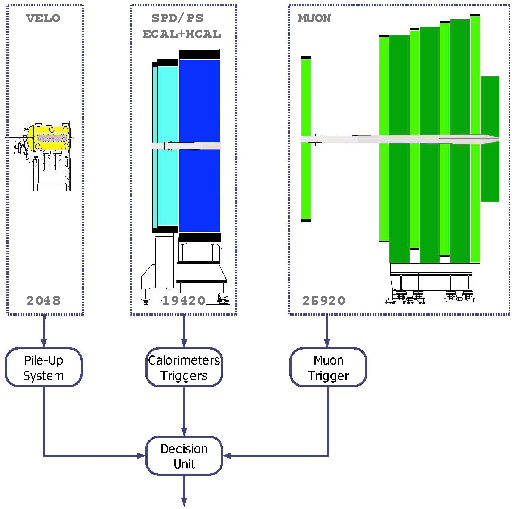
\includegraphics[width=0.6\textwidth]{./figs-detector/trigger/l0_system_schematic.pdf}
    \caption{
        Schematic of the L0 trigger system.
    }
    \label{fig:l0-schematic}
\end{figure}
